% Carbon--SLO research meeting, 18 November 2026.
% Visual system follows 2026-11-11-GreenCache.tex.
% Facts follow the local arXiv PDF (2610.14571v1, 10 Oct 2026).
% Compile with pdfLaTeX from this directory.
\documentclass[aspectratio=169,10pt]{beamer}
\usepackage[english]{babel}
\usepackage[utf8]{inputenc}
\usepackage[T1]{fontenc}
\usepackage{lmodern}
\usepackage{amsmath,amssymb}
\usepackage{booktabs,tabularx,array}
\usepackage{graphicx}
\usepackage{xcolor}
\usepackage{tikz}
\usetikzlibrary{arrows.meta,positioning}

\usetheme{Madrid}
\usecolortheme{default}
\definecolor{Ink}{HTML}{243748}
\definecolor{Muted}{HTML}{667B8B}
\definecolor{Accent}{HTML}{347E74}
\definecolor{AccentBlue}{HTML}{507DAD}
\definecolor{SoftMint}{HTML}{E6F4EE}
\definecolor{SoftLilac}{HTML}{F1EEF8}
\definecolor{Paper}{HTML}{FBFCFE}
\definecolor{Divider}{HTML}{D8E4EB}

\setbeamercolor{background canvas}{bg=Paper}
\setbeamercolor{normal text}{fg=Ink}
\setbeamercolor{structure}{fg=Accent}
\setbeamercolor{frametitle}{fg=Ink,bg=Paper}
\setbeamercolor{title}{fg=Ink}
\setbeamercolor{subtitle}{fg=Muted}
\setbeamercolor{block title}{fg=Ink,bg=Paper}
\setbeamercolor{block body}{fg=Ink,bg=white}
\setbeamercolor{item}{fg=Accent}
\setbeamercolor{footline}{fg=Muted,bg=Paper}
\setbeamercolor{mintbox}{fg=Ink,bg=SoftMint}
\setbeamercolor{bluebox}{fg=Ink,bg=Paper}
\setbeamercolor{lilacbox}{fg=Ink,bg=SoftLilac}
\setbeamerfont{frametitle}{size=\large,series=\bfseries}
\setbeamerfont{footline}{size=\tiny}
\setbeamerfont{block title}{series=\bfseries}
\setbeamertemplate{headline}{}
\setbeamertemplate{navigation symbols}{}
\setbeamertemplate{blocks}[rounded][shadow=false]
\setbeamertemplate{itemize items}[circle]
\setbeamertemplate{enumerate items}[default]
\setbeamertemplate{itemize subitem}[circle]
\newcommand{\slideid}{}
\setbeamertemplate{footline}{%
  \leavevmode\hbox{%
    \begin{beamercolorbox}[wd=\paperwidth,ht=.30cm,dp=.16cm,leftskip=.45cm,rightskip=.45cm]{footline}%
      \insertsectionhead\hfill\hyperlink{INDEX}{Discussion index}\hspace{.40cm}\slideid
    \end{beamercolorbox}}}
\setbeamertemplate{frametitle}{%
  \nointerlineskip
  \begin{beamercolorbox}[wd=\paperwidth,ht=.74cm,dp=.14cm,leftskip=.55cm,rightskip=.40cm]{frametitle}%
    \usebeamerfont{frametitle}\insertframetitle
  \end{beamercolorbox}}
\setbeamersize{text margin left=.48cm,text margin right=.48cm}

\newcommand{\nav}[2]{\hyperlink{#1}{\beamerbutton{#2}}}
\newcommand{\jlink}[1]{\hyperlink{#1}{\textcolor{Accent}{\underline{#1}}}}
\newcommand{\kw}[2]{\hyperlink{#1}{\textcolor{Accent}{\underline{#2}}}}
\newcommand{\slidenote}[1]{\par\vspace{0.05cm}{\scriptsize\color{Muted}Source: Topcu et al., #1}\par}
\newcommand{\back}[2][]{\par\vspace{0.04cm}\nav{#2}{Back to Main \ref*{#2}}\ #1\hfill\nav{INDEX}{Discussion Index}}
\newcommand{\point}[2]{\par\vspace{0.02cm}\textbf{\color{Accent}#1}\quad{\small #2}\par}
\newcommand{\bpoint}[2]{\par\vspace{1.5pt}{\footnotesize\textbf{\color{Accent}#1}\enspace #2}\par}
\newcommand{\takeaway}[1]{%
\vspace{0.05cm}%
\begin{beamercolorbox}[wd=\textwidth,rounded=true,sep=0.07cm]{mintbox}%
{\scriptsize\bfseries\color{Accent}Takeaway}\enspace{\small #1}%
\end{beamercolorbox}}
\newcommand{\card}[3]{%
  \begin{beamercolorbox}[wd=\linewidth,rounded=true,sep=0.07cm]{#1}%
    {\scriptsize\bfseries\color{Accent}#2}\par\vspace{0.4mm}{\small\raggedright #3\par}%
  \end{beamercolorbox}}
\newcommand{\wc}[1]{CarbonSLO-GeoDistributed-LLM-Serving-2026/With-Caption/CarbonSLO_Fig#1.png}
\newcommand{\nc}[1]{CarbonSLO-GeoDistributed-LLM-Serving-2026/Without-Caption/CarbonSLO_Fig#1.png}
% Pixel subsets of the supplied Without-Caption PNGs. Originals are not modified.
\newcommand{\crop}[1]{figures/crops/#1.png}

\title[Carbon--SLO]{Dissecting the Carbon--SLO Tension in Geo-Distributed LLM Serving}
\author{Yu-Jui Liang}
\institute{National Taiwan University / Academia Sinica}
\date{18 Nov 2026}

\begin{document}
\section{Summary}

\renewcommand{\slideid}{Main 01 / 19}
\begin{frame}[c,label=M01]{Carbon--SLO at Geo-Scale}
\vspace*{\fill}
{\LARGE\bfseries Dissecting the Carbon--SLO Tension\par}
{\LARGE\bfseries in Geo-Distributed LLM Serving\par}
\bigskip
{\large Burak Topcu, Musa Cim, Zuhal Ozturk, Mahmut Taylan Kandemir\par}
{\color{Muted}Department of Computer Science and Engineering\\
The Pennsylvania State University\\
arXiv:2610.14571 \quad 10 October 2026}\par\bigskip
\textbf{Research meeting: 18 November 2026}\\
Yu-Jui Liang\quad Advisor: Hsiang-Yun Cheng\\
National Taiwan University / Academia Sinica
\par\vspace{0.35cm}
{\small\color{Muted}Summary \enspace$\cdot$\enspace Motivation \enspace$\cdot$\enspace Simulator \enspace$\cdot$\enspace Four schedulers \enspace$\cdot$\enspace Five results}
\par\vfill
\slidenote{title page.}
\end{frame}

\renewcommand{\slideid}{Main 02 / 19}
\begin{frame}[t,label=M02]{What Does This Paper Do?}
\vspace{0.06cm}
\begin{columns}[T,onlytextwidth]
\begin{column}{0.32\textwidth}
\card{mintbox}{1. Simulator}{\begin{minipage}[t][1.85cm][t]{\dimexpr\linewidth-0.16cm\relax}\raggedright
A geo-distributed LLM serving simulator, calibrated with A100 / vLLM latency and power measurements.\end{minipage}}
\end{column}
\begin{column}{0.32\textwidth}
\card{bluebox}{2. Schedulers}{\begin{minipage}[t][1.85cm][t]{\dimexpr\linewidth-0.16cm\relax}\raggedright
Four carbon- and SLO-aware policies, from a per-request heuristic to a batch-level facility MILP.\end{minipage}}
\end{column}
\begin{column}{0.32\textwidth}
\card{lilacbox}{3. Frontier}{\begin{minipage}[t][1.85cm][t]{\dimexpr\linewidth-0.16cm\relax}\raggedright
The carbon--SLO tradeoff across \kw{B08}{three models}, loads, and carbon-aware and carbon-blind baselines.\end{minipage}}
\end{column}
\end{columns}
\vspace{0.08cm}
\card{bluebox}{Headline result, versus round-robin}{\begin{minipage}[t][1.35cm][t]{\dimexpr\linewidth-0.16cm\relax}\raggedright
Facility MILP reduces \kw{B02}{operational carbon} by \textbf{up to 60\%} relative to round-robin, with the authors' \textbf{average SLO violation of 3\%}. The 60\% is the upper end. The 3\% is an average, not every load.\end{minipage}}
\takeaway{Where a request is served changes both operational carbon and token latency. The lowest-CI site is not automatically the SLO-feasible site.}
\slidenote{Abstract; Sec.~I contributions; Sec.~VIII. The 26--60\% conclusion range is on M19.}
\end{frame}

\section{Motivation}

\renewcommand{\slideid}{Main 03 / 19}
\begin{frame}[t,label=M03]{Why Not Always Choose the Greenest Datacenter?}
\vspace{0.02cm}
{\small\color{Muted}Conceptual schematic, not a measured trace.\par}
\vspace{0.02cm}
\begin{center}
\vspace{-0.15cm}
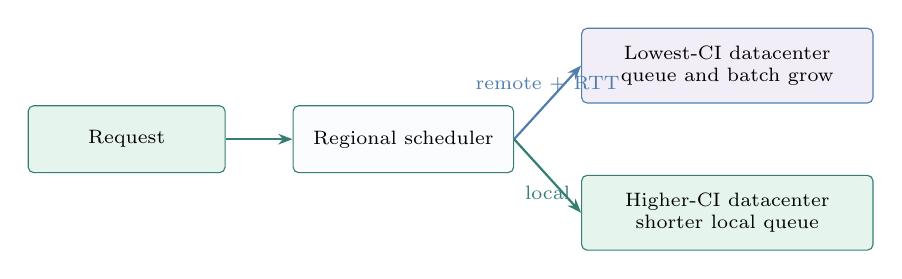
\begin{tikzpicture}[font=\scriptsize, node distance=0.28cm]
  \node[draw=Accent, fill=SoftMint, rounded corners=2pt, align=center, inner sep=3pt, minimum width=2.5cm, minimum height=0.85cm] (req) {Request};
  \node[draw=Accent, fill=Paper, rounded corners=2pt, align=center, inner sep=3pt, minimum width=2.8cm, minimum height=0.85cm, right=0.85cm of req] (sch) {Regional scheduler};
  \node[draw=AccentBlue, fill=SoftLilac, rounded corners=2pt, align=center, inner sep=3pt, minimum width=3.7cm, minimum height=0.95cm, above right=0.02cm and 0.85cm of sch] (low) {Lowest-CI datacenter\\queue and batch grow};
  \node[draw=Accent, fill=SoftMint, rounded corners=2pt, align=center, inner sep=3pt, minimum width=3.7cm, minimum height=0.95cm, below right=0.02cm and 0.85cm of sch] (high) {Higher-CI datacenter\\shorter local queue};
  \draw[-{Stealth[length=1.8mm]}, thick, Accent] (req) -- (sch);
  \draw[-{Stealth[length=1.8mm]}, thick, AccentBlue] (sch.east) -- node[above, font=\scriptsize] {remote + RTT} (low.west);
  \draw[-{Stealth[length=1.8mm]}, thick, Accent] (sch.east) -- node[below, font=\scriptsize] {local} (high.west);
\end{tikzpicture}
\vspace{-0.25cm}
\end{center}
\point{Carbon opportunity}{\kw{B02}{Carbon intensity} varies by more than an order of magnitude across regions and time. Routing toward a lower-CI grid cuts operational carbon.}
\point{Latency cost}{A crowd of requests raises queueing and TTFT, and a larger decode batch raises TPOT. The remote path also pays network RTT.}
\takeaway{Minimum CI and the SLO-feasible assignment are different decisions once queueing, batching, and RTT are counted.}
\slidenote{Sec.~I, paragraphs on spatial scheduling; Sec.~II, CI variation. Source-mix medians are on the backup.}
\end{frame}

\renewcommand{\slideid}{Main 04 / 19}
\begin{frame}[t,label=M04]{What Do Previous Approaches Miss?}
\vspace{0.08cm}
{\small \kw{B01}{Table I} compares six carbon-aware geo-scheduling studies with this paper. The gaps are not identical for every row.\par}
\vspace{0.10cm}
\begin{columns}[T,onlytextwidth]
\begin{column}{0.49\textwidth}
\card{lilacbox}{Load-independent latency}{\begin{minipage}[t][1.35cm][t]{\dimexpr\linewidth-0.16cm\relax}\raggedright
Most coarse plans (SLIT, Green-LLM, FREESH, MARLIN) treat latency as independent of the live batch. MOER is per request, but it has no latency target.\end{minipage}}
\vspace{0.06cm}
\card{bluebox}{Phase-dependent power}{\begin{minipage}[t][1.12cm][t]{\dimexpr\linewidth-0.16cm\relax}\raggedright
None fully models prefill versus decode power. MOER is marked partial. The others are unmarked.\end{minipage}}
\end{column}
\begin{column}{0.49\textwidth}
\card{lilacbox}{Queue, KV admission, network}{\begin{minipage}[t][1.35cm][t]{\dimexpr\linewidth-0.16cm\relax}\raggedright
None models engine queueing when KV memory or the batch slot is full. FREESH and MOER also omit inter-region transfer; several others include it.\end{minipage}}
\vspace{0.06cm}
\card{bluebox}{Which latency SLO?}{\begin{minipage}[t][1.12cm][t]{\dimexpr\linewidth-0.16cm\relax}\raggedright
Prior targets are mostly self-defined: mean TTFT, a 5\,s end-to-end cap, or job wait. This paper uses TTFT and TPOT against MLPerf budgets.\end{minipage}}
\end{column}
\end{columns}
\takeaway{The open question is load-dependent TTFT and TPOT under a benchmark SLO, not a new carbon signal by itself.}
\slidenote{Sec.~I and Table~I. GCOS is a GPU-job scheduler; its latency column is not a token SLO.}
\end{frame}

\section{Problem}

\renewcommand{\slideid}{Main 05 / 19}
\begin{frame}[t,label=M05]{What Is the Carbon--SLO Scheduling Problem?}
\vspace{0.04cm}
{\small The decision is which datacenter receives the request. It is not a transfer of layers, KV cache, or MoE experts.\par}
\vspace{0.02cm}
\[
\mathrm{CO_2}=\sum_{d\in D} E_d\cdot \mathrm{CI}_d,
\qquad
E_d=\mathrm{PUE}_d\int P_d(t)\,dt
\]
\vspace{-0.25cm}
{\centering\footnotesize $P_d$ sums host power and per-engine power. One PUE and one CI per datacenter.\par}
\vspace{0.08cm}
\begin{columns}[T,onlytextwidth]
\begin{column}{0.49\textwidth}
\card{mintbox}{Operational carbon only}{\begin{minipage}[t][1.45cm][t]{\dimexpr\linewidth-0.18cm\relax}\raggedright
Scope~2 electricity emissions. This paper does not optimize embodied carbon, and it does not trade model quality.\end{minipage}}
\end{column}
\begin{column}{0.49\textwidth}
\card{lilacbox}{\kw{B02}{SLO violation}}{\begin{minipage}[t][1.45cm][t]{\dimexpr\linewidth-0.18cm\relax}\raggedright
A request violates the SLO if \textbf{either} TTFT or TPOT exceeds its budget. Main budgets: 3\,s and 100\,ms; Mixtral TPOT is 200\,ms.\end{minipage}}
\end{column}
\end{columns}
\takeaway{Carbon is energy times grid intensity, with PUE. Latency is two separate token budgets, and missing either one counts.}
\slidenote{Sec.~II, GHG Protocol and problem formulation; Table~II budgets. MLPerf's original TTFT is 2\,s; they relax it for geo delay.}
\end{frame}

\section{Simulator}

\renewcommand{\slideid}{Main 06 / 19}
\begin{frame}[t,label=M06]{How Does the Geo-Distributed Simulator Work?}
\vspace{0.02cm}
\begin{columns}[T,onlytextwidth]
\begin{column}{0.60\textwidth}
\centering\includegraphics[width=\linewidth,height=4.55cm,keepaspectratio]{\wc{03}}
\end{column}
\begin{column}{0.38\textwidth}
\vspace{0.08cm}
{\scriptsize\bfseries\color{Accent}Figure 3, numbered path}\par\vspace{0.08cm}
{\footnotesize
\textbf{1.} Load generator sends a Poisson request to a regional scheduler.\par\vspace{0.06cm}
\textbf{2--3.} The scheduler keeps it local or forwards it. A remote hop pays RTT, then the peer scheduler places it.\par\vspace{0.06cm}
\textbf{4--5.} The provisioner polls each datacenter and broadcasts the snapshot plus the RTT matrix.\par\vspace{0.08cm}
Inside a datacenter, inter-node and intra-node placement are round-robin. The engine runs \kw{B05}{continuous batching}.\par}
\end{column}
\end{columns}
\takeaway{Scheduling sees a polled per-datacenter snapshot: batch size, queue depth, KV occupancy, prefill duty, and CI.}
\slidenote{Sec.~III-C, Fig.~3; Sec.~III-A for the polled fields. Savings are attributed to the regional policy because intra-DC placement is round-robin.}
\end{frame}

\renewcommand{\slideid}{Main 07 / 19}
\begin{frame}[t,label=M07]{How Is LLM Serving Latency Modeled?}
\vspace{0.02cm}
{\centering\includegraphics[width=\linewidth,height=2.68cm,keepaspectratio]{\wc{01}}\par}
\vspace{0.01cm}
\point{Prefill, Fig.~1(a)}{Nearly flat for short prompts, then roughly linear in prefill tokens. A constant TTFT cannot represent that knee.}
\point{Decode, Fig.~1(b)}{Sublinear in batch size, then sharp after saturation, and higher when the KV context is longer.}
\point{Fit, Fig.~1(c)}{An \kw{B03}{analytical model} calibrated on A100 / vLLM measurements. Held-out MAPE is within 1.7\% (dense prefill), 4.8\% (Mixtral prefill), and 3.4\% (decode).}
\takeaway{TTFT and TPOT are functions of the live batch, the queue, and the context. They are not constants the scheduler can look up once.}
\slidenote{Sec.~III-B, Fig.~1. Coefficients and the exact polynomials are on the backup.}
\end{frame}

\renewcommand{\slideid}{Main 08 / 19}
\begin{frame}[t,label=M08]{How Are Power and Energy Modeled?}
\vspace{0.02cm}
\begin{columns}[T,onlytextwidth]
\begin{column}{0.56\textwidth}
\centering\includegraphics[width=\linewidth,height=4.35cm,keepaspectratio]{\wc{02}}
\end{column}
\begin{column}{0.42\textwidth}
\vspace{0.10cm}
\point{Two curves}{Prefill power reaches TDP once the prompt is long enough. Decode power grows with batch size and stays more sensitive to load.}
\point{Energy}{Each step is average power times step latency. A fast, high-power prefill and a long, lower-power decode do not cost the same.}
\point{Always on}{The \kw{B03}{power model} also charges about 72\,W per idle A100 and 300\,W of host power. Idle GPUs are not free carbon.}
\end{column}
\end{columns}
\takeaway{Load-dependent energy is part of the carbon price. A scheduler that ignores phase and batch will mis-rank datacenters.}
\slidenote{Sec.~III-B, Fig.~2. Held-out step energy is within 5.6\% MAPE. TDP shown is 400\,W for the A100.}
\end{frame}

\renewcommand{\slideid}{Main 09 / 19}
\begin{frame}[t,label=M09]{Real GPUs or a Simulator? How Is It Validated?}
\vspace{0.06cm}
\begin{columns}[T,onlytextwidth]
\begin{column}{0.32\textwidth}
\card{mintbox}{A. Real hardware}{\begin{minipage}[t][1.35cm][t]{\dimexpr\linewidth-0.16cm\relax}\raggedright
A100-40GB, vLLM v0.6.3, FP16. Latency and power are profiled on this GPU.\end{minipage}}
\end{column}
\begin{column}{0.32\textwidth}
\card{bluebox}{B. Analytical fit}{\begin{minipage}[t][1.35cm][t]{\dimexpr\linewidth-0.16cm\relax}\raggedright
Per-phase latency and energy models, one fit per model and tensor-parallel degree.\end{minipage}}
\end{column}
\begin{column}{0.32\textwidth}
\card{lilacbox}{C. Geo-simulation}{\begin{minipage}[t][1.35cm][t]{\dimexpr\linewidth-0.16cm\relax}\raggedright
Many regions, schedulers, queues, RTT, and carbon. This layer is not another hardware run.\end{minipage}}
\end{column}
\end{columns}
\vspace{0.06cm}
\card{bluebox}{\kw{B04}{Within-node validation}, Llama-3.1-8B only}{\begin{minipage}[t][1.15cm][t]{\dimexpr\linewidth-0.16cm\relax}\raggedright
Three data-parallel vLLM engines, 19 arrival rates, more than 40K requests. TPOT average error below 5\%. TTFT average error 9.1\%. GPU energy within 2.5\% of the measurement.\end{minipage}}
\vspace{0.06cm}
\card{lilacbox}{What this does not certify}{\begin{minipage}[t][1.05cm][t]{\dimexpr\linewidth-0.16cm\relax}\raggedright
The check is single-node inference serving. It is not a validation that 16 physical datacenters were deployed. Mixtral at TP=4 already fills their four-GPU node.\end{minipage}}
\slidenote{Sec.~V-B; limitations in Sec.~VI. TTFT error is 3.5\% below saturation, 5.2\% in overload, and 28.5\% near saturation.}
\end{frame}

\section{Method}

\renewcommand{\slideid}{Main 10 / 19}
\begin{frame}[t,label=M10]{Which Scheduling Policies Are Proposed?}
\vspace{0.04cm}
{\small All four share one latency estimator. They differ in how many requests they decide together, and in how they price energy.\par}
\vspace{0.06cm}
{\centering\scriptsize
\setlength{\tabcolsep}{4pt}
\renewcommand{\arraystretch}{1.18}
\begin{tabular}{@{}llll@{}}
\toprule
Policy & Decision & Load coupling & Energy of a batch \\
\midrule
\kw{B06}{Greedy} heuristic & one request & current snapshot only & not shared \\
Standard ILP & one window, one solve & frozen inside that solve & sum of per-request costs \\
Iterative ILP & same window, up to 3 solves & re-projected after each solve & still additive \\
\kw{B07}{Facility MILP} & window, plus a use bit per DC & capacity gated by that bit & wake-up charged once \\
\bottomrule
\end{tabular}\par}
\vspace{0.10cm}
\point{Greedy $\alpha{=}0$}{Carbon only. The paper states that this coincides with MOER. $\alpha{=}1$ would be latency only. They report 0, 0.5, and 0.9.}
\point{Why the ladder}{Each step is aimed at one failure of the previous step: uncoordinated requests, a stale load estimate, then double-counted batch energy.}
\takeaway{Facility MILP is not only a larger ILP. It changes who pays the shared energy of a batch.}
\slidenote{Sec.~IV opening and Sec.~IV-A--C. Solver limits: $T_{\max}{=}3$, MILP time limit 0.25\,s, HiGHS.}
\end{frame}

\renewcommand{\slideid}{Main 11 / 19}
\begin{frame}[t,label=M11]{How Do Greedy and Standard ILP Work?}
\vspace{0.04cm}
\begin{columns}[T,onlytextwidth]
\begin{column}{0.49\textwidth}
\card{mintbox}{Greedy, per request}{\begin{minipage}[t][3.35cm][t]{\dimexpr\linewidth-0.18cm\relax}\raggedright
Keep only SLO-feasible datacenters, then
\[
\alpha\,\widehat{\mathrm{Lat}}+(1{-}\alpha)\,\widehat{\mathrm{CI}}.
\]
Latency is TTFT plus OSL times TPOT. Hats divide by the max over feasible datacenters. The request goes to the lowest score.\par\vspace{0.08cm}
Weakness: requests in the same polling period herd onto one site. Concurrent schedulers share one snapshot.\end{minipage}}
\end{column}
\begin{column}{0.49\textwidth}
\card{bluebox}{Standard ILP, one window}{\begin{minipage}[t][3.35cm][t]{\dimexpr\linewidth-0.18cm\relax}\raggedright
Assign the window jointly:
\[
\min\sum c_{r,d}x_{r,d},\quad
\sum_d x_{r,d}=1,\quad
\sum_r x_{r,d}\le H_d.
\]
$c_{r,d}=\mathrm{PUE}_d\,E_{r,d}\,\mathrm{CI}_d$. $H_d$ is remaining batch slots.\par\vspace{0.08cm}
The \kw{B06}{full ILP} freezes $H_d$ and the latency estimates for that single solve.\end{minipage}}
\end{column}
\end{columns}
\takeaway{Greedy cannot coordinate a window. Standard ILP can, but it still prices every request against the load from before the assignment.}
\slidenote{Sec.~IV-A, Eq.~(1); Sec.~IV-B, Eq.~(2). Window: 100\,ms or 300 requests. The matrix is totally unimodular.}
\end{frame}

\renewcommand{\slideid}{Main 12 / 19}
\begin{frame}[t,label=M12]{Why Iterative ILP and Facility MILP?}
\vspace{0.05cm}
\begin{columns}[T,onlytextwidth]
\begin{column}{0.49\textwidth}
\card{lilacbox}{Iterative ILP}{\begin{minipage}[t][2.15cm][t]{\dimexpr\linewidth-0.18cm\relax}
Write the assignment back into each datacenter's batch and queue, recompute TTFT and TPOT, and solve again. Stop on a repeated assignment or after 3 iterations.\end{minipage}}
\end{column}
\begin{column}{0.49\textwidth}
\card{mintbox}{Facility MILP}{\begin{minipage}[t][2.15cm][t]{\dimexpr\linewidth-0.18cm\relax}
Add a one-time carbon $f_d$ if datacenter $d$ receives any request in the window. Marginal request energy stays in $c_{r,d}$.\end{minipage}}
\end{column}
\end{columns}
\vspace{0.08cm}
{\centering
\setlength{\abovedisplayskip}{2pt}\setlength{\belowdisplayskip}{2pt}
\(\displaystyle
\min\sum c_{r,d}x_{r,d}+\sum_d f_d y_d,
\qquad
\sum_r x_{r,d}\le H_d y_d,
\qquad y_d\in\{0,1\}
\)\par}
\vspace{0.04cm}
{\small An additive model can charge an idle engine's fixed step energy twice when two requests share that batch. The $y_d$ term charges that \kw{B07}{shared batch energy} once.\par}
\takeaway{The MILP changes the energy model of a shared batch. It does not power off a datacenter, and it does not remove RTT.}
\slidenote{Sec.~IV-B--C. $f_d$ is the carbon of waking $d$'s engines for the window, not a measured facility shutdown.}
\end{frame}

\section{Experiments}

\renewcommand{\slideid}{Main 13 / 19}
\begin{frame}[t,label=M13]{How Is the System Evaluated?}
\vspace{0.04cm}
{\centering\scriptsize
\setlength{\tabcolsep}{5pt}
\renewcommand{\arraystretch}{1.12}
\begin{tabular}{@{}lll@{}}
\toprule
 & Dense & MoE \\
\midrule
Models & Llama-3.1-8B, Qwen2.5-7B, TP=1 & Mixtral-8x7B, top-2 of 8, TP=4 \\
Token budgets & TTFT 3\,s, TPOT 100\,ms & TTFT 3\,s, TPOT 200\,ms \\
Arrival rate & 1200 / 2400 / 4000 req/s & 800 / 1200 / 2000 req/s \\
Engines per DC & 32 (4 nodes $\times$ 8 GPUs) & 8, because each engine uses 4 GPUs \\
\bottomrule
\end{tabular}\par}
\vspace{0.08cm}
\point{Topology}{4 regional schedulers $\times$ 4 datacenters $=$ 16 DCs. RTT 85--280\,ms. Default PUE 1.1. CI is an Electricity Maps hour, held fixed inside a run. \kw{B08}{Table II} has the full list.}
\point{Baselines}{Carbon-blind: round-robin and least-loaded. Carbon-aware: Green-LLM, and MOER, which matches greedy at $\alpha{=}0$.}
\point{Metrics}{Operational carbon in gCO$_2$, including idle and host energy. SLO violation rate. Also TTFT p50 / p90 / p99, because the violation rate hides the tail.}
\takeaway{The 16 datacenters are simulated roles on one server, not a 16-site hardware deployment. Dense and MoE do not have the same engine count.}
\slidenote{Sec.~V-A, Table~II. Load labels: low / moderate / high are under 15\%, 15--40\%, and above 40\% of batch capacity under round-robin.}
\end{frame}

\renewcommand{\slideid}{Main 14 / 19}
\begin{frame}[t,label=M14]{Q1: Can Carbon Be Reduced Without Excessive SLO Violations?}
\vspace{0.01cm}
{\centering\scriptsize Figure 4(a), Topcu et al. Y: carbon saving versus round-robin. X: fraction of requests missing TTFT or TPOT.\par}
\vspace{0.01cm}
{\centering\includegraphics[height=3.72cm]{\crop{fig4a}}\par}
\vspace{0.02cm}
\takeaway{Facility MILP keeps most of the carbon saving at a low violation rate. Carbon-only greedy matches the saving only by spending the SLO.}
\vspace{0.05cm}
{\scriptsize\textbf{How to read the claim.} Up to 60\% and the average 3\% SLO violation are the authors' summary versus \kw{B08}{baselines} RR, not the coordinate of every marker. Low load is omitted from this figure: facility MILP saves 53.8--59.6\% there. The most carbon-aggressive greedy setting reaches up to 55\% violation; that is not true of greedy at $\alpha{=}0.9$.\par}
\slidenote{Abstract; Sec.~V-C, Fig.~4(a). Moderate-load $\alpha{=}0$: up to 6.9\% violation on dense models and 44.8\% on Mixtral.}
\end{frame}

\renewcommand{\slideid}{Main 15 / 19}
\begin{frame}[t,label=M15]{Q2: What Happens to Tail Latency Under High Load?}
\vspace{0.01cm}
{\centering\scriptsize Figure 4(b), Topcu et al., high load only. Bars are TTFT from p50 to p99. The printed percentages are carbon savings versus RR, not latency.\par}
\vspace{0.01cm}
{\centering\includegraphics[height=2.98cm]{\crop{fig4b}}\par}
\vspace{0.01cm}
\point{Dense models}{Greedy keeps p99 TTFT inside 3\,s, but $\alpha{=}0$ still fails the SLO on TPOT: decode batches sit on the green datacenters.}
\point{Mixtral}{Greedy $\alpha{=}0$ pushes median TTFT to 3.3\,s. ILP and MILP keep the median within 0.7\,s and p99 within 2.2\,s. Aggressive greedy and Green-LLM reach p99 up to 8.8\,s.}
\takeaway{A reasonable median is not a tail inside the SLO, and a TTFT tail inside the budget is not a passed \kw{B02}{SLO violation rate}.}
\slidenote{Sec.~V-C, Fig.~4(b). Iterative ILP p99 TTFT reaches 7.5\,s on the dense models, from repeated solves.}
\end{frame}

\renewcommand{\slideid}{Main 16 / 19}
\begin{frame}[t,label=M16]{Q3: How Do PUE and Carbon-Intensity Spread Affect Savings?}
\vspace{0.02cm}
{\centering\scriptsize Figure 5, Topcu et al. (a)~high-load PUE. (b)~facility MILP across CI hours. Open versus filled markers in (a): uniform PUE 1.1 versus real per-DC PUE.\par}
\vspace{0.02cm}
\begin{columns}[T,onlytextwidth]
\begin{column}{0.42\textwidth}
\centering\includegraphics[height=3.55cm]{\crop{fig5a}}\\[0.06cm]
{\scriptsize Real PUE is 1.08--1.32. Facility MILP moves from 29.2\% to 30.5\% (Llama) and 36.6\% to 38.7\% (Mixtral). SLO barely changes.\par}
\end{column}
\begin{column}{0.56\textwidth}
\centering\includegraphics[height=3.55cm]{\crop{fig5b}}\\[0.06cm]
{\scriptsize From the lowest CV (0.31) to the highest (0.94), savings rise and the SLO stays flat. High load still saves up to 39--45\% when the spread is large.\par}
\end{column}
\end{columns}
\takeaway{A wider \kw{B09}{PUE and CI spread} creates the carbon opportunity. Higher load spends it. PUE mostly rescales carbon, not the SLO.}
\slidenote{Sec.~V-C, Fig.~5. The 13\% Llama point at high load and the lowest CV is outside the conclusion's 26--60\% summary.}
\end{frame}

\renewcommand{\slideid}{Main 17 / 19}
\begin{frame}[t,label=M17]{Q4: How Important Are Polling, Overhead, and Topology?}
\vspace{0.01cm}
{\centering\scriptsize Figure 6, Topcu et al. (a)~scheduler CPU time at high load. (b)~facility-MILP SLO violation at moderate load. (c)~Llama, high load.\par}
\vspace{0.01cm}
\begin{columns}[T,onlytextwidth]
\begin{column}{0.64\textwidth}
\centering\includegraphics[width=\linewidth,height=4.15cm,keepaspectratio]{\nc{06}}
\end{column}
\begin{column}{0.34\textwidth}
\vspace{0.02cm}
{\scriptsize\bfseries\color{Accent}(a) Solver $\neq$ GPU}\par
{\scriptsize Greedy is under 1\,ms. Facility MILP p99 is up to 0.5\,s. Iterative ILP p99 is 6.5\,s on Llama.\par}
\vspace{0.08cm}
{\scriptsize\bfseries\color{Accent}(b) \kw{B09}{Polling period}}\par
{\scriptsize At most 2\,s: violation stays at most 8.2\%. At 5\,s it rises to 10.5--32\%.\par}
\vspace{0.08cm}
{\scriptsize\bfseries\color{Accent}(c) Topology}\par
{\scriptsize Eight schedulers: violation 10.3\% to 19.4\%. Fewer, larger DCs: violation 4.1\%, saving 23.2\%.\par}
\end{column}
\end{columns}
\takeaway{Token SLO tracks how fresh the load snapshot is. The milliseconds and seconds in panel (a) are scheduler time, not TTFT.}
\slidenote{Sec.~V-C, Fig.~6. Asynchronous polling does not consistently beat synchronous polling.}
\end{frame}

\renewcommand{\slideid}{Main 18 / 19}
\begin{frame}[t,label=M18]{Q5: What If Output Length Is Unknown?}
\vspace{0.01cm}
{\centering\scriptsize Figure 7, Topcu et al. (a)~high load, oracle versus predicted OSL. (b)~Mixtral prompt length as batch capacity grows.\par}
\vspace{0.01cm}
\begin{columns}[T,onlytextwidth]
\begin{column}{0.62\textwidth}
\centering\includegraphics[width=\linewidth,height=4.05cm,keepaspectratio]{\nc{07}}
\end{column}
\begin{column}{0.36\textwidth}
\vspace{0.04cm}
{\scriptsize\bfseries\color{Accent}Why OSL is in the score}\par
{\scriptsize Decode time and decode energy scale with output length. The paper's example: OSL 100 occupies an engine about 10$\times$ longer than OSL 10.\par}
\vspace{0.08cm}
{\scriptsize\bfseries\color{Accent}\kw{B09}{Predicted OSL}}\par
{\scriptsize Savings move by at most 1.3 points on Llama and 4.1 on Mixtral. Violations rise by at most 1.1 points, except iterative ILP on Llama.\par}
\vspace{0.08cm}
{\scriptsize\bfseries\color{Accent}Longer prompts}\par
{\scriptsize Near a 5\% violation, facility MILP still saves up to 30\% (long) and 28\% (mixed).\par}
\end{column}
\end{columns}
\takeaway{These policies tolerate a rough output-length estimate. The carbon--SLO result does not require the oracle length.}
\slidenote{Sec.~IV and Sec.~V-C, Fig.~7. Exact-bucket accuracy is only 51\% (Llama) and 37\% (Mixtral); adjacent buckets cover 99\% and 70\%.}
\end{frame}

\section{Conclusion}

\renewcommand{\slideid}{Main 19 / 19}
\begin{frame}[t,label=M19]{Conclusion}
\vspace{0.02cm}
\card{bluebox}{1. Problem}{Chasing a lower-CI datacenter moves TTFT and TPOT through queueing, batching, and RTT.}
\vspace{0.05cm}
\card{mintbox}{2. Contribution}{A within-node-calibrated simulator and four schedulers. Facility MILP prices shared batch energy instead of summing isolated requests.}
\vspace{0.05cm}
\card{bluebox}{3. Evidence}{Versus round-robin: up to 60\% less operational carbon, average SLO violation 3\%. Savings grow with CI spread, shrink with load, and depend on snapshot freshness.}
\vspace{0.05cm}
\card{lilacbox}{4. \kw{B10}{Limitations}, and what is not this paper}{Not done here: multi-turn KV locality and heterogeneous hardware. Our direction --- heterogeneous GPUs, HBM/HBF, attention and expert placement, cross-DC carbon-aware serving --- is not an author result.}
\slidenote{Sec.~VI and Sec.~VIII. The conclusion's 26--60\% band is across loads at the base setting; Fig.~5(b) leaves that band when the CI hour changes.}
\end{frame}

\section{Index}

\renewcommand{\slideid}{Index}
\begin{frame}[t,label=INDEX]{Discussion Index}
\vspace{0.02cm}
{\small Main is the talk. This index opens the evidence behind a question.\par}
\vspace{0.06cm}
{\scriptsize
\setlength{\tabcolsep}{3.5pt}
\renewcommand{\arraystretch}{1.08}
\begin{tabularx}{\textwidth}{@{}lXl@{}}
\toprule
Topic & What is here & Jump \\
\midrule
Gap & Table~I, row by row, including partial cells & \jlink{B01} \\
\noalign{\vskip 4pt}
Definitions & CI, PUE, Scope~2, TTFT, TPOT, violation & \jlink{B02} \\
\noalign{\vskip 4pt}
Step models & Latency and energy formulas, MAPE, idle power & \jlink{B03} \\
\noalign{\vskip 4pt}
Validation & 19 rates, error by regime, single-node limit & \jlink{B04} \\
\noalign{\vskip 4pt}
Engine & Continuous batching, KV admission, queueing & \jlink{B05} \\
\noalign{\vskip 4pt}
Greedy / ILP & Equation~(1), Equation~(2), frozen load & \jlink{B06} \\
\noalign{\vskip 4pt}
MILP & Iteration, wake-up bit, what $y_d$ does not do & \jlink{B07} \\
\noalign{\vskip 4pt}
Setup & Table~II, baselines, load labels, not 16 real sites & \jlink{B08} \\
\noalign{\vskip 4pt}
Sensitivity & PUE, CV, polling, topology, OSL, prompt length & \jlink{B09} \\
\noalign{\vskip 4pt}
Limits & Reproducibility and claims we would not make & \jlink{B10} \\
\bottomrule
\end{tabularx}\par}
\vspace{0.08cm}
{\small
\textbf{Simulator trust} \nav{M09}{M09} \nav{B04}{B04}
\quad
\textbf{Main result} \nav{M14}{M14} \nav{M15}{M15}
\quad
\textbf{Method} \nav{M12}{M12} \nav{B07}{B07}\par}
\vspace{0.06cm}
\nav{M19}{Go to Conclusion (M19)}\hfill\nav{INDEX}{Discussion Index}
\end{frame}

\section{Backup}

\renewcommand{\slideid}{B01}
\begin{frame}[t,label=B01]{Table I: What Each Prior Scheduler Models}
\vspace{0.02cm}
{\scriptsize Check marks follow Table~I: modeled, not modeled, partial, or not applicable. ``Ours'' is this paper.\par}
\vspace{0.04cm}
{\centering\scriptsize
\setlength{\tabcolsep}{2.6pt}
\renewcommand{\arraystretch}{0.92}
\begin{tabular}{@{}l>{\raggedright\arraybackslash}p{3.55cm}>{\raggedright\arraybackslash}p{4.15cm}l@{}}
\toprule
Study & Placement and latency target & Lat.\ / power / queue / transfer & Reported \\
\midrule
SLIT & 15-min plan; min TTFT, unbounded & no / no / no / yes & mean TTFT \\
Green-LLM & 1-hour plan; mean E2E $\le$ 5\,s & no / no / no / yes & none (\$ penalty) \\
FREESH & 30-min plan; E2E $\le$ 5$\times$ profiled & no / no / no / no & E2E viol., p99 \\
GCOS & per GPU-job; wait $\le$ 10--20\% runtime & n/a / no / no / yes & wait violation \\
MARLIN & 15-min plan; min TTFT, unbounded & no / no / no / yes & mean TTFT \\
MOER & per request; no latency target & no / partial / no / no & E2E p95 \\
Ours & per request and batch; TTFT and TPOT at MLPerf & yes / yes / yes / yes & SLO, p50/90/99 \\
\bottomrule
\end{tabular}\par}
\vspace{0.06cm}
\point{Do not flatten the column}{``Most'' of the coarse planners assume load-independent latency. That sentence in Sec.~I cites SLIT, Green-LLM, FREESH, and MARLIN. It is not a claim that MOER or GCOS make the same latency assumption.}
\point{Transfer is mixed}{Queueing from KV admission is unmarked for every prior row. Inter-region transfer is marked for SLIT, Green-LLM, GCOS, and MARLIN, and unmarked for FREESH and MOER.}
\slidenote{Sec.~I, Table~I.}
\back{M04}
\end{frame}

\renewcommand{\slideid}{B02}
\begin{frame}[t,label=B02]{Carbon Accounting, TTFT, TPOT, and the SLO}
\vspace{0.02cm}
\point{Carbon intensity}{Generation-weighted: $\mathrm{CI}=\sum_g (P_g/P_{\mathrm{total}})\cdot \mathrm{CI}_g$. The paper quotes median CI below 50\,gCO$_2$/kWh for nuclear and solar, 490 for natural gas, and 820 for coal. CI varies by more than an order of magnitude across regions and time.}
\point{Scope 2}{Operational emissions over intervals are $\sum_k E_{\mathrm{tot}}[k]\cdot \mathrm{CI}[k]$, with $E_{\mathrm{tot}}=P_{\mathrm{tot}}\Delta t$ and $P_{\mathrm{tot}}=P_{\mathrm{IT}}\times \mathrm{PUE}$. Across datacenters, $\mathrm{CO_2}=\sum_d E_d\cdot \mathrm{CI}_d$.}
\point{Inside one datacenter}{$E_d=\mathrm{PUE}_d\int P_d(t)\,dt$ and $P_d$ adds host power to every engine's power. One PUE and one CI per datacenter, because the site shares the grid and the facility.}
\point{TTFT}{Queueing plus prefill, plus scheduling delay and inter-region RTT when the placement is remote.}
\point{TPOT}{Average decode-step time, including steps stalled by another request's prefill.}
\point{SLO violation}{The fraction of requests that miss either the TTFT budget or the TPOT budget. Main study: 3000\,ms / 100\,ms. Mixtral TPOT is 200\,ms. Long and mixed prompts use a 4500\,ms TTFT. MLPerf's single-node TTFT is 2\,s; only TTFT is relaxed.}
\point{Not this paper's objective}{No embodied-carbon term, no SSD amortization, and no quality-for-carbon trade.}
\slidenote{Sec.~II; Table~II; Sec.~III-A.}
\back[\nav{M02}{Main 2} \nav{M03}{Main 3} \nav{M15}{Main 15}]{M05}
\end{frame}

\renewcommand{\slideid}{B03}
\begin{frame}[t,label=B03]{Analytical Latency and Power Formulas}
\vspace{0.02cm}
{\scriptsize
\setlength{\abovedisplayskip}{2pt}
\setlength{\belowdisplayskip}{1pt}
\setlength{\abovedisplayshortskip}{1pt}
\setlength{\belowdisplayshortskip}{1pt}
Prefill time, for total tokens $N$, batch $B$, and prompt lengths $n_i$:
\[
t_{\mathrm{pre}}=t_{\mathrm{tok}}(N)+b_0+b_1 B+b_2\sum_i n_i^2 .
\]
$t_{\mathrm{tok}}$ is piecewise linear in $N$. Its slope increases after a saturation point $k$.

Decode time is quadratic in batch size. Each coefficient is linear in the mean cached length $\ell=K/B$:
\[
t_{\mathrm{dec}}=a_0+a_1 B+a_2 B^2,\qquad a_j=\alpha_j+\beta_j \ell .
\]
Step energy, not power alone:
\[
E_{\mathrm{pre}}=e^{\mathrm{pre}}_0+e_p N+e_a\sum_i n_i^2,
\qquad
E_{\mathrm{dec}}=e^{\mathrm{dec}}_0+e_d B+e_k K .
\]
\par}
\vspace{0.02cm}
\point{MAPE}{Prefill step time: within 1.7\% for Llama-3.1-8B and Qwen2.5-7B at both TP degrees, and 4.8\% for Mixtral-8x7B at TP=4. Decode step time: within 3.4\% on all five setups. Held-out step energy: within 5.6\%.}
\point{Standing power}{Idle engine: about 72\,W per A100. Host: 300\,W, of which the CPU package is about 146\,W under load on their testbed. Calibration: vLLM v0.6.3, FP16, A100, prompts from 32 to 32K tokens.}
\point{Why decode MAPE is the weaker fit}{Decode steps are tens of milliseconds, so thermal and frequency transients show up. The paper states that limit.}
\slidenote{Sec.~III-B, Figs.~1--2. Symbols follow the paper's prose; the PDF does not number these displays as equations.}
\back[\nav{M08}{Main 8}]{M07}
\end{frame}

\renewcommand{\slideid}{B04}
\begin{frame}[t,label=B04]{Within-Node Validation, and Its Boundary}
\vspace{0.02cm}
\point{What was replayed}{Three data-parallel Llama-3.1-8B vLLM engines, TP=1, A100-40GB, CNN-DailyMail, round-robin, Poisson rates from 2 to 50 req/s. The simulator then replays each logged engine, arrival time, input length, and actual output length.}
\point{Where those rates sit}{Measured saturated capacity is 27.58 req/s. The sweep covers 7\% to 181\% of that capacity, including the queue-free regime and overload.}
\point{Errors, 19 rates, more than 40K requests}{TPOT moves from 15.5\,ms to 54\,ms as prefills stall decode; average error is below 5\%. TTFT moves from 71\,ms to more than 20\,s; overall average error is 9.1\%. Split: 3.5\% below saturation, 5.2\% in overload, 28.5\% around saturation, where the simulator overestimates TTFT.}
\point{Independence and energy}{One engine instead of three, at the same per-engine load, changes TPOT by 3.3\%. Simulated GPU energy stays within 2.5\% of the measurement at every rate.}
\point{Boundary}{Sec.~VI: validation is within a node and for Llama-3.1-8B only. A single Mixtral-8x7B engine at TP=4 already fills the four-GPU node, so Mixtral has no matching multi-engine end-to-end check. Absolute carbon on other GPUs would move. The 16-datacenter experiments remain simulation.}
\slidenote{Sec.~V-B and Sec.~VI. Step-model MAPE in Sec.~III-B is a separate check from this end-to-end replay.}
\back{M09}
\end{frame}

\renewcommand{\slideid}{B05}
\begin{frame}[t,label=B05]{Continuous Batching, KV Capacity, and Queueing}
\vspace{0.04cm}
\bpoint{Admission}{Each step retires finished requests, then admits queued ones while the batch limit and the new KV both fit. Queueing delay depends on occupancy. It is not a fixed constant.}
\bpoint{Engine budgets}{Batch size follows vLLM \texttt{max\_num\_seqs}; the per-step token budget follows \texttt{max\_num\_batched\_tokens}. A long prefill is split across steps and stalls the running decode batch.}
\bpoint{KV example}{Llama-3.1-8B uses 128\,KiB of KV per token after the weights. Batch capacity is 40 at TP=1, 80 at TP=2, and 400 for Mixtral.}
\bpoint{TTFT estimate}{Scheduling delay, RTT if remote, wait for a slot, and prefill: $\mathrm{TTFT}_{r,d}=\mathrm{RTT}(s,s')+W_d+t_{\mathrm{pre}}(\mathrm{ISL}_r+Q_d)$.}
\bpoint{TPOT estimate}{$\mathrm{TPOT}_{r,d}=t_{\mathrm{dec}}(B_d{+}1,\mathrm{KV}_d)+T^{\mathrm{pre}}_d/(1-\mathrm{duty}_d)$. The $+1$ is this request. Duty stretches decode by prefills already running.}
\bpoint{Per-datacenter snapshot}{The provisioner polls batch size, queue tokens, KV occupancy, prefill duty, and CI. The paper uses averages so the poll and the decision stay small.}
\slidenote{Sec.~III-C and the latency estimator in Sec.~IV. Intra-DC schedulers are round-robin.}
\back{M06}
\end{frame}

\renewcommand{\slideid}{B06}
\begin{frame}[t,label=B06]{Greedy Score and the Standard ILP}
\vspace{0.01cm}
{\scriptsize Equation~(1). $\mathcal{F}_r$ is the set of datacenters whose estimated TTFT and TPOT meet the SLO. $\mathrm{Lat}_{r,d}=\mathrm{TTFT}_{r,d}+\mathrm{OSL}_r\cdot\mathrm{TPOT}_{r,d}$.
\[
\mathrm{score}_{r,d}
=\alpha\frac{\mathrm{Lat}_{r,d}}{\max_{d'\in\mathcal{F}_r}\mathrm{Lat}_{r,d'}}
+(1-\alpha)\frac{\mathrm{CI}_d}{\max_{d'\in\mathcal{F}_r}\mathrm{CI}_{d'}} .
\]
$\alpha{=}0$ is carbon only and matches MOER. $\alpha{=}1$ is latency only. Reported settings are 0, 0.5, and 0.9. Herding: every request in a polling period can select the same site, and regional schedulers act on one shared snapshot.\par}
\vspace{0.02cm}
{\scriptsize Equation~(2). $x_{r,d}\in\{0,1\}$, $c_{r,d}=\mathrm{PUE}_d\cdot E_{r,d}\cdot\mathrm{CI}_d$, and $H_d=\max(0,\mathrm{cap}_d-\mathrm{load}_d)$.
\[
\min_x \sum_{r\in R}\sum_{d\in\mathcal{F}_r} c_{r,d}x_{r,d}
\quad\text{s.t.}\quad
\sum_{d\in\mathcal{F}_r} x_{r,d}=1,\quad
\sum_{r\in R} x_{r,d}\le H_d .
\]
The constraint matrix is totally unimodular, so the LP relaxation is integral. HiGHS solves it in tens of milliseconds. $H_d$ and the latency estimates stay fixed during this one solve: a datacenter that is feasible for each request alone can miss the SLO after the requests land together.\par}
\vspace{0.04cm}
\point{Fallback}{If the solver fails or cannot place a request inside capacity, the scheduler uses the lowest-CI SLO-feasible datacenter with headroom, which is greedy at $\alpha{=}0$, and round-robin if none exists.}
\point{OSL}{Both TPOT's queued-prefill term and the carbon estimate need the output length. The main experiments use the oracle length. The predicted length is only the Fig.~7 study.}
\slidenote{Sec.~IV-A--B, Eqs.~(1)--(2); Sec.~V-A fallback and OSL.}
\back[\nav{M10}{Main 10}]{M11}
\end{frame}

\renewcommand{\slideid}{B07}
\begin{frame}[t,label=B07]{Iterative ILP and the Facility MILP}
\vspace{0.02cm}
\point{What iteration updates}{After solve $t$, $n^{(t)}_d=\sum_r x^{(t)}_{r,d}$ is projected onto that datacenter's batch size and queue as if the window had already been dispatched. TTFT, TPOT, the feasible set, and $E_{r,d}$ are recomputed. Equation~(2) is solved again until two successive assignments match or $T_{\max}=3$.}
\point{What iteration does not change}{Carbon is still a sum of per-request costs. Capacity and latency constraints couple the requests. The energy model does not.}
\point{Wake-up bit}{The facility MILP adds $\sum_d f_d y_d$ to the objective and replaces the capacity row with $\sum_r x_{r,d}\le H_d y_d$, $y_d\in\{0,1\}$. $y_d=1$ means $d$ receives at least one request from the window. $f_d$ is the carbon of waking $d$'s engines. Two requests on an idle engine then pay that fixed step energy once, not twice.}
\point{Size of the extra model}{Only $|D|$ new binaries, against $|R|\cdot|D|$ assignment variables. The paper says HiGHS still finishes inside the 0.25\,s limit.}
\point{Does not power off}{This is an accounting device for shared batch energy inside the window. It does not power off a datacenter building, it does not delete inter-region RTT, and idle engines still remain in the later discussion of engine activation.}
\slidenote{Sec.~IV-B--C. The engine-activator remark in Sec.~VI is an observation, not a claim that the MILP already implements it.}
\back[\nav{M10}{Main 10}]{M12}
\end{frame}

\renewcommand{\slideid}{B08}
\begin{frame}[t,label=B08]{Table II, Baselines, and Load Labels}
\vspace{0.02cm}
{\scriptsize
\setlength{\tabcolsep}{3pt}
\renewcommand{\arraystretch}{0.88}
\begin{tabular}{@{}lp{10.6cm}@{}}
\toprule
Item & Value in the paper \\
\midrule
Regions & 4 schedulers: EU-North, US-East, Asia, South America. 4 DCs each. EU-North examples: Netherlands, Belgium, Lithuania, Latvia. \\
Hardware roles & 4 nodes per DC, 8$\times$ A100-40GB per node. Simulated. The sweep runs on one 64-core server, 200\,s per policy-rate pair. \\
Network and PUE & Inter-region RTT 85--280\,ms, AWS one-year p50. Default PUE 1.1. Real per-DC PUE is only the Fig.~5(a) sweep. \\
CI & Electricity Maps, hourly, held constant within a run. \\
Load labels & Mean round-robin batch / batch capacity: low $<$15\%, moderate 15--40\%, high $>$40\%. Rates 1200/2400/4000 (7B/8B) and 800/1200/2000 (Mixtral). \\
Models & Llama-3.1-8B and Qwen2.5-7B are dense, TP=1. Mixtral-8x7B is MoE, 13B active, TP=4, so a quarter as many engines per DC. \\
Scheduler knobs & Poll 1\,s (swept 0.5--10\,s). Window 100\,ms or 300 requests. Greedy $\alpha\in\{0,0.5,0.9\}$. Oracle OSL except Fig.~7. \\
\bottomrule
\end{tabular}\par}
\vspace{0.05cm}
\bpoint{Round-robin and least-loaded}{Carbon-blind, one request at a time. Intra-DC placement is also round-robin, so measured savings are credited to the regional scheduler.}
\bpoint{Green-LLM and MOER}{Green-LLM is ported as scheduling decisions only. MOER sends each request to the lowest-CI SLO-feasible datacenter, which is greedy at $\alpha{=}0$.}
\bpoint{Not a 16-site deployment}{No claim in the PDF says these 16 datacenters were physically built for the experiment.}
\slidenote{Sec.~V-A, Table~II.}
\back[\nav{M02}{Main 2} \nav{M14}{Main 14}]{M13}
\end{frame}

\renewcommand{\slideid}{B09}
\begin{frame}[t,label=B09]{Figure 5--7: Values Behind the Charts}
\vspace{0.01cm}
{\scriptsize Panels are on Main 16--18. Savings below are versus round-robin. Sec.~V-C.\par}
\vspace{0.02cm}
\begin{columns}[T,onlytextwidth]
\begin{column}{0.49\textwidth}
\bpoint{PUE, high load}{Reported PUE 1.08 (Netherlands) to 1.32 (Japan). Facility MILP: Llama 29.2\% to 30.5\%, Mixtral 36.6\% to 38.7\%. Japan in this note is CI 449--502 with PUE 1.32. SLO barely moves. These baselines are not the 26\% / 35\% labels on Fig.~4(b); the PDF does not reconcile them.}
\bpoint{CI spread}{35K hours, 2021--2024. CV 0.31 to 0.94. Llama/Mixtral: low 49/44\% to 59/55\%; moderate 34/39\% to 56/55\%; high 13/24\% to 39/45\%. SLO flat. The 13\% point is outside the 26--60\% conclusion sentence.}
\bpoint{Overhead, polling}{Greedy $<$1\,ms. Facility MILP p99 up to 0.5\,s. Iterative ILP p99 6.5\,s on Llama. Poll $\le$2\,s: violation at most 8.2\%. At 5\,s: 10.5--32\%. Async is not consistently better.}
\end{column}
\begin{column}{0.49\textwidth}
\bpoint{Topology}{Llama, high load, facility MILP. Doubling schedulers: violation 10.3\% to 19.4\%, savings almost unchanged. Fewer, larger DCs: violation 4.1\%, saving 23.2\%. Engine count is matched.}
\bpoint{Predicted OSL}{MLP, 128 units, about 27K parameters, $<$0.1\,ms. Exact bucket 51\% Llama and 37\% Mixtral (random guess 17\%). Adjacent included: 99\% and 70\%. Savings move $\le$1.3 and $\le$4.1 points. Violations $\le$1.1 points, except iterative ILP on Llama.}
\bpoint{GovReport and mixed prompts}{Mean ISL 10.7K at 50 req/s, and 2.9K at 200 req/s. TTFT budget 4.5\,s. Facility MILP saves up to 30\% at batch capacity 16 (long) and 28\% at 24 (mixed), near 5\% violation.}
\end{column}
\end{columns}
\slidenote{Sec.~V-C, Figs.~5--7. Fig.~4(b) labels and the PUE paragraph are both quoted; they are not averaged together.}
\back[\nav{M17}{Main 17} \nav{M18}{Main 18}]{M16}
\end{frame}

\renewcommand{\slideid}{B10}
\begin{frame}[t,label=B10]{Limits, Reproducibility, and Open Questions}
\vspace{0.02cm}
\begin{columns}[T,onlytextwidth]
\begin{column}{0.49\textwidth}
\bpoint{What the PDF shows}{A calibrated simulator and a scheduling comparison under MLPerf-derived token SLOs. The carbon result is versus round-robin, stated as an average and as a frontier, not as one guaranteed point.}
\bpoint{Validation}{Within a node, Llama-3.1-8B, three engines. Not a 16-datacenter hardware deployment. Other GPUs would change absolute latency and carbon. The authors expect the queueing pattern to carry over, and they do not show that.}
\bpoint{Workload}{Single-turn requests. Long prompts stress KV capacity. Multi-turn sessions, where prefix KV ties the next turn to one datacenter, are future work in the paper.}
\end{column}
\begin{column}{0.49\textwidth}
\bpoint{Not an extra system}{Facility MILP leaves Llama TP=1 engines idle 73\% / 56\% / 33\% of the time at low / moderate / high load, versus at most 10\% for round-robin. Idle plus host energy is 28--81\% of remaining carbon. The engine activator is only motivated. At TP=2, facility MILP emits 22\% more carbon at high load.}
\bpoint{Our direction}{Heterogeneous GPUs, HBM/HBF, attention and expert placement, and cross-datacenter carbon-aware serving. Our direction is not an author result.}
\bpoint{Reproducibility}{Code: \texttt{github.com/topcuburak/carbon-slo-at-geoscale}. This deck does not re-run it. If the repository and the PDF disagree, the PDF remains the source of these claims.}
\end{column}
\end{columns}
\slidenote{Sec.~VI and Sec.~VIII. Claude assistance is disclosed by the authors in the acknowledgment; they say the technical claims are theirs.}
\back{M19}
\end{frame}

\end{document}
